\documentclass[12pt]{article}

\usepackage{mystyle}

\title{\textbf{IB Internal Assessment}\\\textbf{Physics SL}\\ Measuring the efficiency of wind turbines}

%\pagestyle{fancy}
%\fancyhead{}
%\fancyfoot{}
%
%\fancyhead[L]{\tiny Agnes H\o y-Thomsen\\Physics SL\\Candidate Number: 000115-0026}
%\fancyfoot[C]{\thepage}

\begin{document}

\maketitle

%AGNES: START WRITING HERE
\section{Introduction} 

Climate change has been a heavily debated issue the past couple of years, with increasing concern for the future of humanity.
With the poles melting and sea levels rising as well as the ozone layer disappearing and the planet heating up, many species are now in danger of extinction.
Sea levels is a problem I particularly worry about in my country, Denmark, which is surrounded by oceans, has a flat surface, and already struggles with sea slowly eroding the coast lines.
With fossil fuels being \SI{87}{\percent} of the world's primary energy consumption, according to a study in 2012, it's clear that alternatives to fossil fuels are not very efficient \cite{FossilFuels}.
Besides this argument,  emission not only affects the environment, but also our health; we seem to care more about short-term profits than our and the next generations' health.
Nuclear power is an alternative producing enormous amounts of energy, but the radiation released is highly dangerous and waste material has to be hidden deep ground or in mountains.

Renewable energy is increasing every year and lots of money is invested in new technology to improve the world's savers in the future.
Not only does renewable energy help reducing the global warming, it also uses sources that are free and practically infinite.
I focused on wind turbines and how efficient they are, as they are one of the alternatives to fossil fuels.
It is an interesting topic, since it is such of current importance and this will hopefully increase my area of knowledge about wind turbines and their function in our world, and therefore, I will investigate the efficiency of wind turbines.


\section{Background Theory}

The sun emits radiation, some of which is absorbed by the surface of the Earth absorbs and therefore the surface heats up.
However, due to many reasons the temperature increase is different in different locations.
Where the temperature is higher, the air rises and creates low pressure.
Places with cooler temperatures have denser air do not rise, therefore creating high pressure.
The movement of air from high to low pressure is an example of convectional currents and creates wind.

Albert Betz discovered the maximum theoretical output of a wind turbine being \SI{59,3}{\percent}, which is known as Betz's Coefficient \cite{Betz}.
However, this is a theoretical output.
It is estimated more realistically that a wind turbine, under Danish weather circumstances, only uses and converts an average of \SIrange{25}{30}{\percent} of the actual energy available to it throughout the year, yet modern turbines can use up to \SI{45}{\percent} of the wind on optimal days.
However, due to around \SIrange{6}{10}{\percent} loss of energy in the gearbox and the generator, the realistic average of power is between \SIrange{22}{28}{\percent} \cite{WindTurbineWorks}.

\begin{equation}
  P = \frac{1}{2} \rho A \vec{v}^{\,3}
  \label{equation:Windpower}
\end{equation}

Equation \ref{equation:Windpower} is the power of the wind that reaches the turbines within the area of the wings, which is quite useful, since not all wind goes to the turbine, but only that within the area.
$P$ is power, $\rho$ is air density, $A$ is the area of the blades with $r$ being the length of one blade, and $v$ is the velocity of the wind.
The average wind speed for it to turn is around \SIrange{6}{8}{\metre\per\second} throughout the year.
This equation can be seen as the input of the turbine and is measured in Watts (\si{\watt}).

\begin{equation}
  P=VI
  \label{equation:Power}
\end{equation}

Equation \ref{equation:Power} is another formula to calculate power, where $P$ is power, $V$ is voltage and $I$ is current.
This formula says that if voltage and current is multiplied it gives power, which is also measured in Watts (\si{\watt}).

\begin{equation}
  R = \frac{V}{I}
  \label{equation:Ohmslaw}
\end{equation}

In a circuit, we can calculate the resistance, where $R$ is resistance, $V$ is voltage and $I$ is current.
It is measured in Ohms (\si{\ohm}).

\subsection{Mechanics}
The wind makes the blades turn the main shaft converting kinetic energy into mechanical energy.
The gearbox gets the speed up to 3000 rotations per minute, which is \SI{50}{\hertz}.
Then it goes to the generator, which converts mechanical into electric energy.

The blades are bent backwards slightly to make the wind push the blades down to make them turn.
The winds can be pitched regulated in order to control power output.
This means that the wings can turn to reach a specific angle between the blade and the wind, the pitch angle.
This makes the efficiency of the turbine constant during high wind speeds over \SI{14}{\metre\per\second}.
Even though it does not drop in efficiency it does, however, mean that even though the wind speed increases with more than \SI{14}{\metre\per\second}, the turbine does not utilise the extra power input it gets.
For stall regulation, the blades cannot be turned, which then gives less energy extraction and the efficiency drops, when wind speeds are high, but protects the turbine from breaking and also does not need active control.
For wind speeds over \SI{20}{\metre\per\second}, the turbines shut down due to safety measures.

Figure \ref{figure:OfficialTurbine} shows the effects of stalling and pitching through various wind speeds and is called the ``wind turbine power curve''.
The blue line is stall-regulated and the red line is pitch-regulated.
The graph shows that the blue line can take a bit more wind speed and produce maximum power, where as it then decreases with higher wind speeds.
The red line reaches a maximum speed and stays constant instead of decreasing, which usually is desired rather than for it to decrease like the blue one.

\begin{figure}[h]
  \centering
  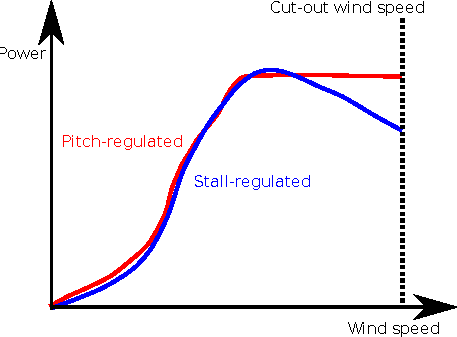
\includegraphics[width=0.5\textwidth]{img/WindTurbine.pdf}
  \caption{Graph showing Power and Wind Speed with Stall and Pitch regulated blades.}
  \label{figure:OfficialTurbine}
\end{figure}

\subsection{Electromagnetic Induction}
In order to understand how the turbine generates electricity, electromagnetic induction is important, since a generator is being used in this experiment.
Inside the generator there is a magnetic field.
An electric coil moves a magnetic field and through that a voltage is induced and an electric circuit is created.
The faster the conductor or coil moves the bigger voltage induced.
In a DC motor, the wires are changed via a commutator in order to get a rectified voltage.
In wind turbines there is usually an electromagnet inside the generator, however in the bigger turbines a permanent magnet is secured, which creates its own magnetic field without the use of current from the turbine.
A difference is that electromagnetism costs energy to maintain a field.

Lorentz' Force Law is the force that affects a charged particle in an electromagnetic field, due to the electric field and the magnetic field.

\begin{equation}
  F = q \vec{E} + q \vec{v} \times \vec{B}
\end{equation}

$F$ is the force, $q$ is the electric charge, $\vec{E}$ is the electric field, $\vec{v}$ is velocity and $\vec{B}$ is the magnetic field. 
This is relevant since it shows that the faster a rotation of the motor is, the more power, due to the velocity.

\subsection{Efficiency}

For this experiment the power will be what the turbine produces on the voltmeter and ammeter and is the product of voltage and current.
The input is the power from the air coming in the area of the turbine.
The efficiency is measured as a percentage.

It is important to keep in mind that of all the power in the area of the turbine blades, a maximum of \SI{45}{\percent} of that power is actually used and average is \SIrange{22}{28}{\percent}.
Since my turbine is far from an optimal one, I would estimate the percentage to be even lower.

\section{Method and Data Analysis}

The equipment used for this experiment was:
\begin{itemize}
  \item 2 Fans (\SI{28}{\watt} each)
  \item A self made wind turbine
  \item Voltmeter 
  \item Ammeter 
  \item Ruler
  \item Microsoft Excel
  \item Thermometer
  \item App on phone for wind speed
\end{itemize}

The dependent variable is voltage and current, since they are affected by the wind speed or distance from the fan to the turbine.
Since power is the product of the two variables that is also changing.

Independent variable is the distance, but can also be the wind speed as they relate to each other.
My controlled variable is temperature and air pressure, and the fans continue to blow the air at the same speed, and the volt and ammeter are noted every 10 seconds.

For this experiment I decided to build my own wind turbine: I crafted it from PVC wires, a DC motor and some wire.
With a soldering iron I soldered the wire together with the DC motor, seen in \ref{figure:soldering}, and pulled it through the PVC frame.
A wooden cylinder was glued onto the motor and through that three holes where drilled for the blades.
The wings are made of card and bent slightly for them to catch more wind.
I tried wooden blades as well, but they were too heavy for this experiment and could not turn.
It should be mentioned that were no safety issues involving this experiment.

\begin{figure}[h]
  \centering
  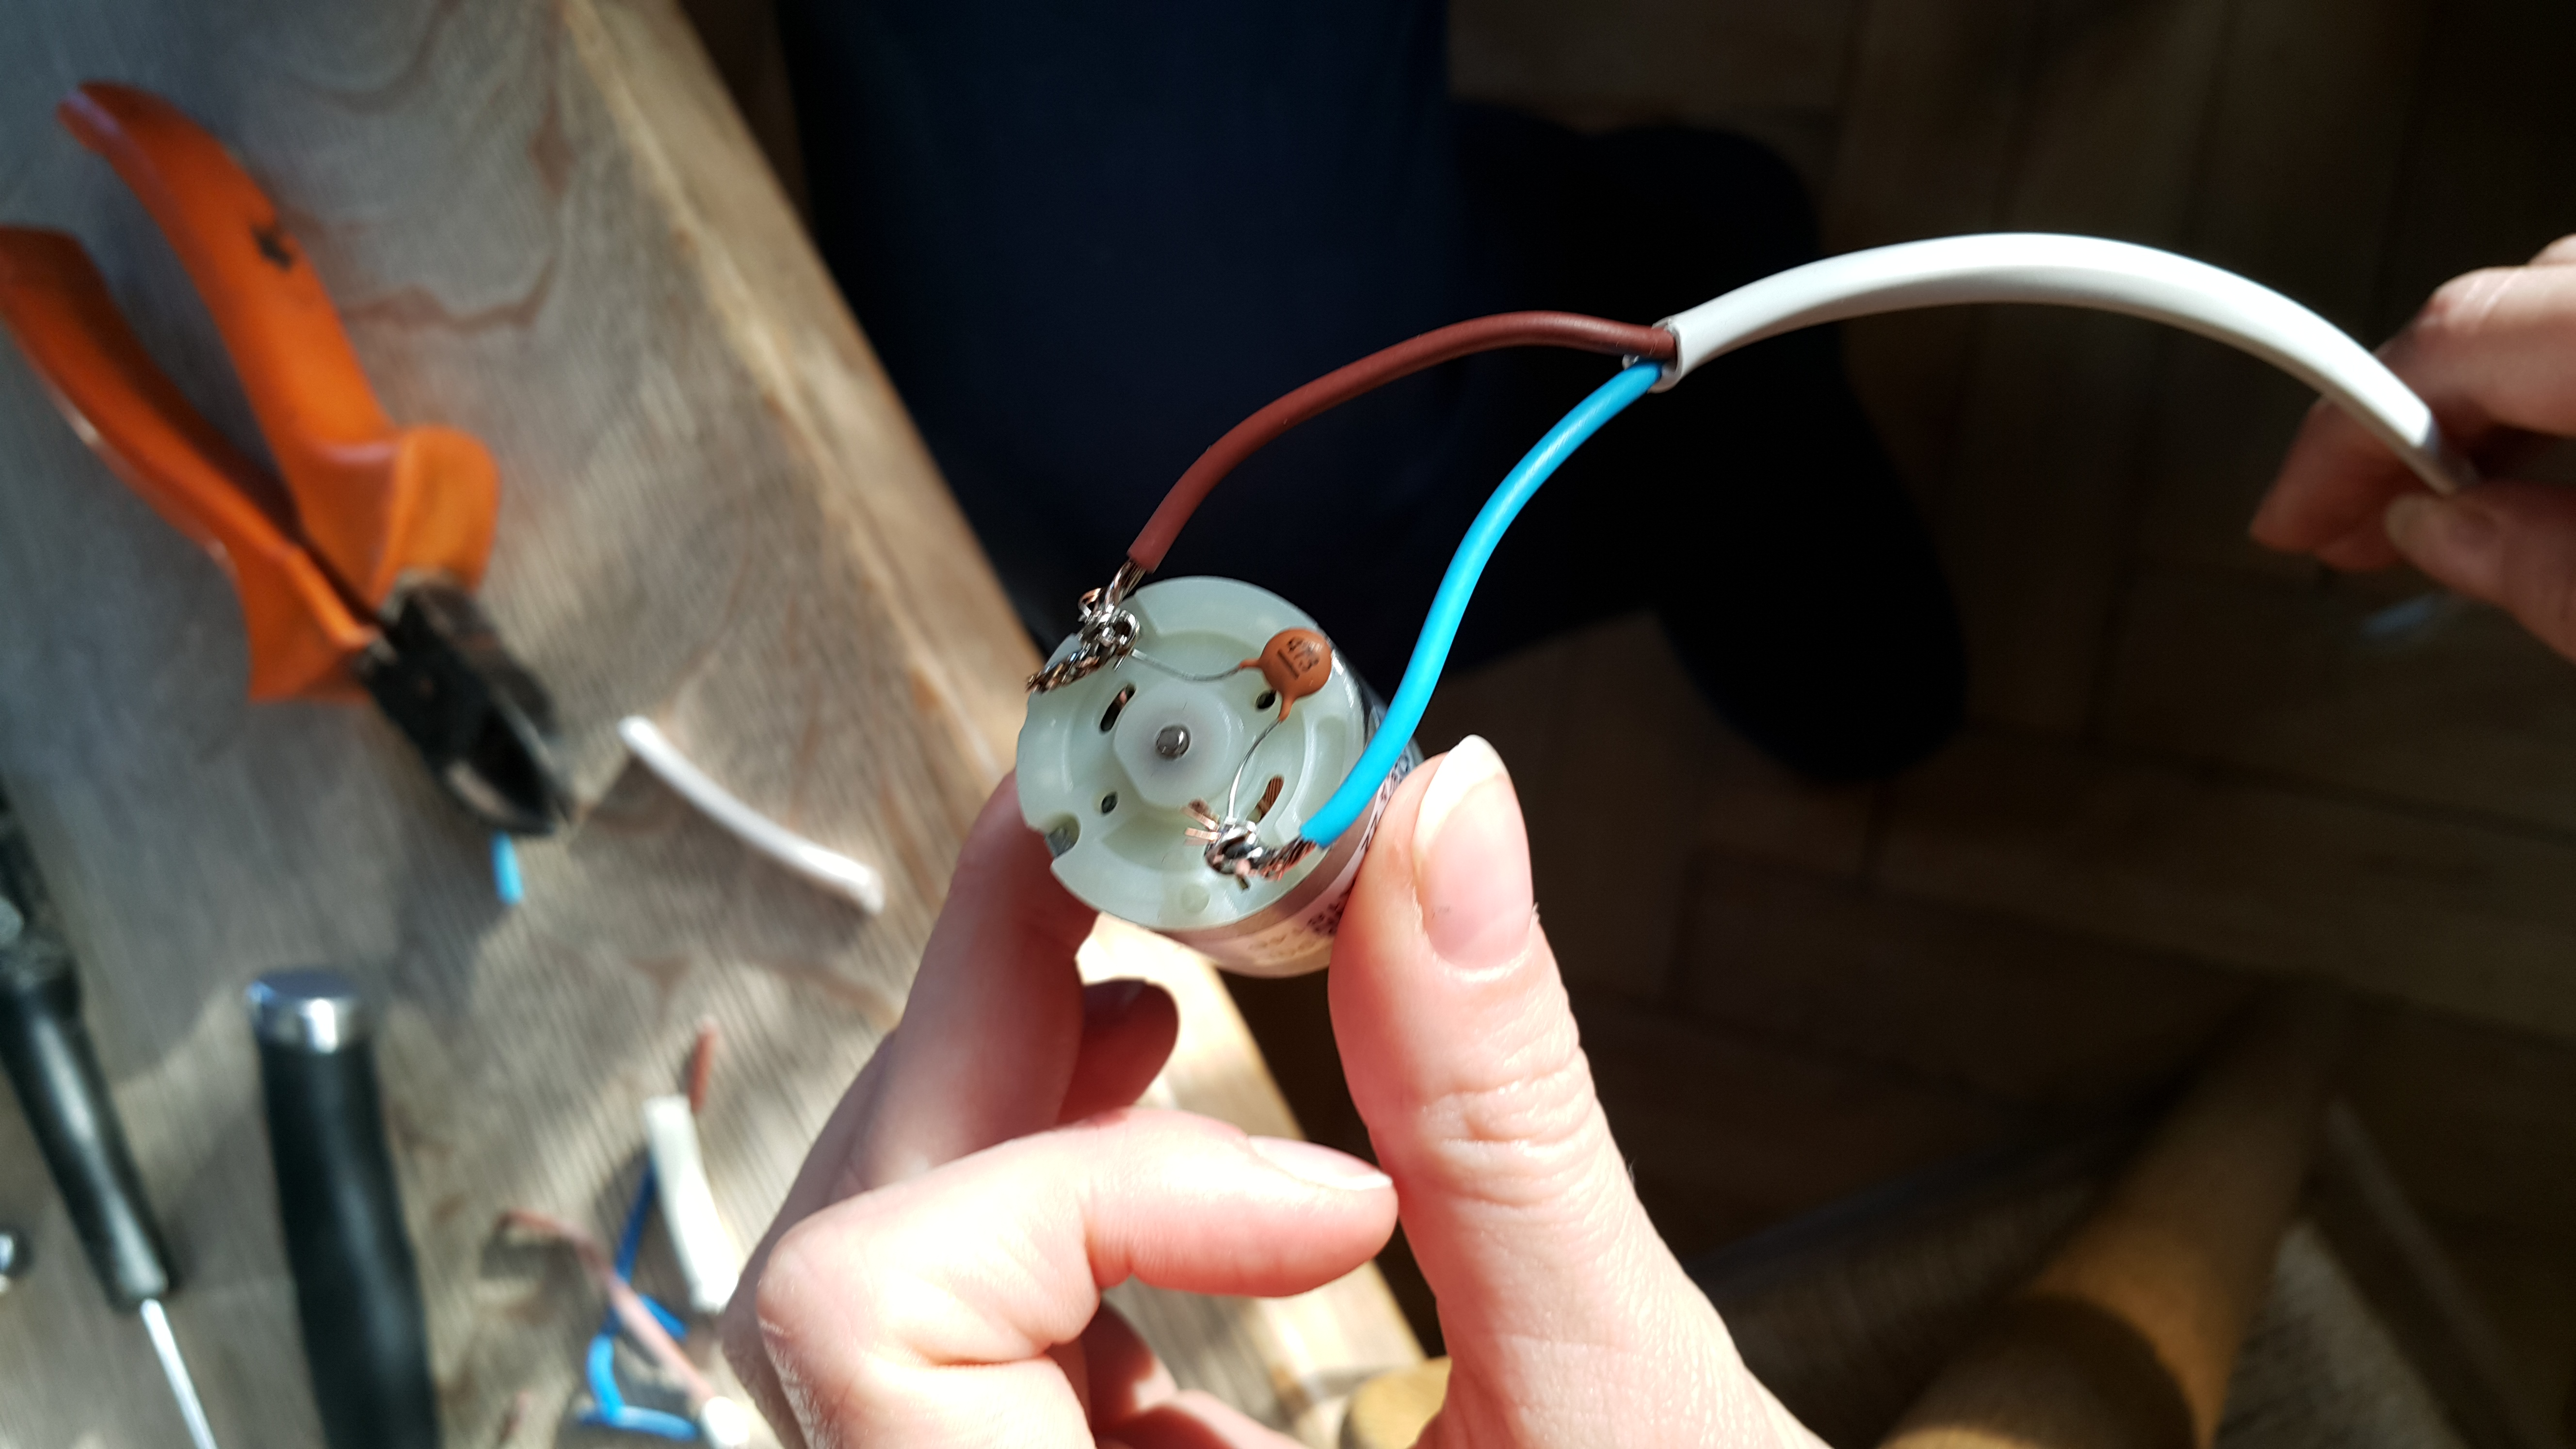
\includegraphics[width=0.5\textwidth]{img/solder.jpg}
  \caption{Soldering the wires to the DC motor.}
  \label{figure:soldering}
\end{figure}
\begin{figure}[h]
  \centering
  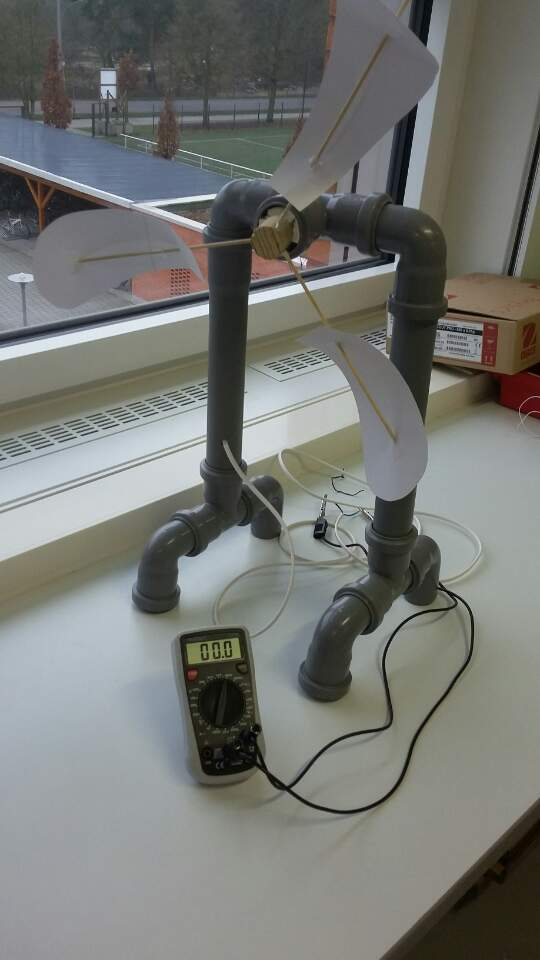
\includegraphics[width=0.25\textwidth]{img/turbine.jpg}
  \caption{My finished wind turbine.}
  \label{figure:MyWindTurbine}
\end{figure}

I set up my experiment in the following way: two fans were placed on boxes in order for them to set the air off in the right height for the turbine.
A voltmeter and an ammeter were placed in circuit with the wire from the turbine.
For this experiment I measured 10 different distances from the fan to the turbine.
This was to be able to regulate the speed of the wind in order to see if the power outcome changes dependent on wind speed.

\begin{figure}[h]
  \centering
  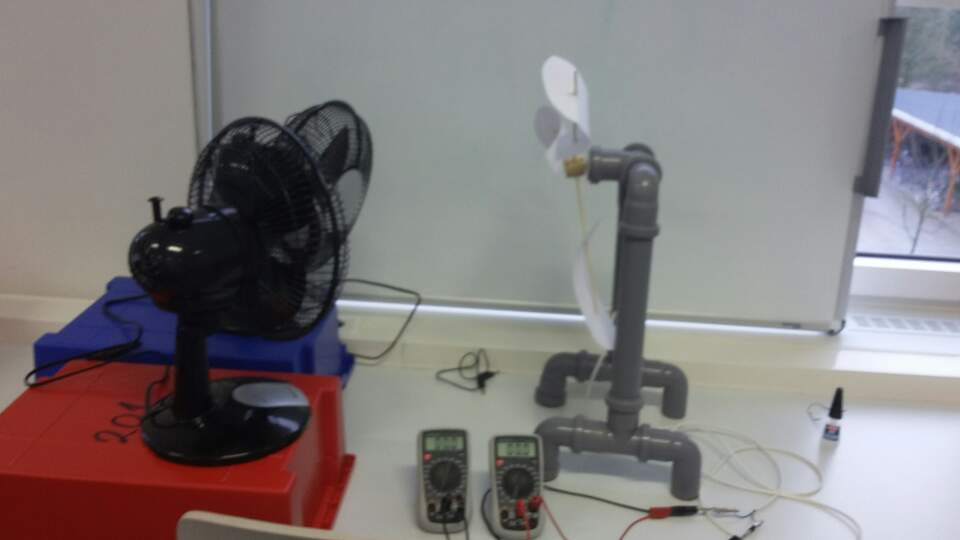
\includegraphics[width=0.5\textwidth]{img/finalsetup.jpg}
  \caption{The final set up of the experiment.}
  \label{figure:FinalSetup}
\end{figure}

For each distance I measured the average wind speed, since the app used for measurement on the phone sensed different speeds at a very high rate and then displayed the average every second, where I kept the device until the average was constant for more than 20 seconds.
The distance was always measured from the edge of the blue box to the front of the feet of the turbine, which can be seen in the picture above.
I plotted a graph to prove the relationship between the distance and the wind speed:

\begin{figure}[h]
\centering
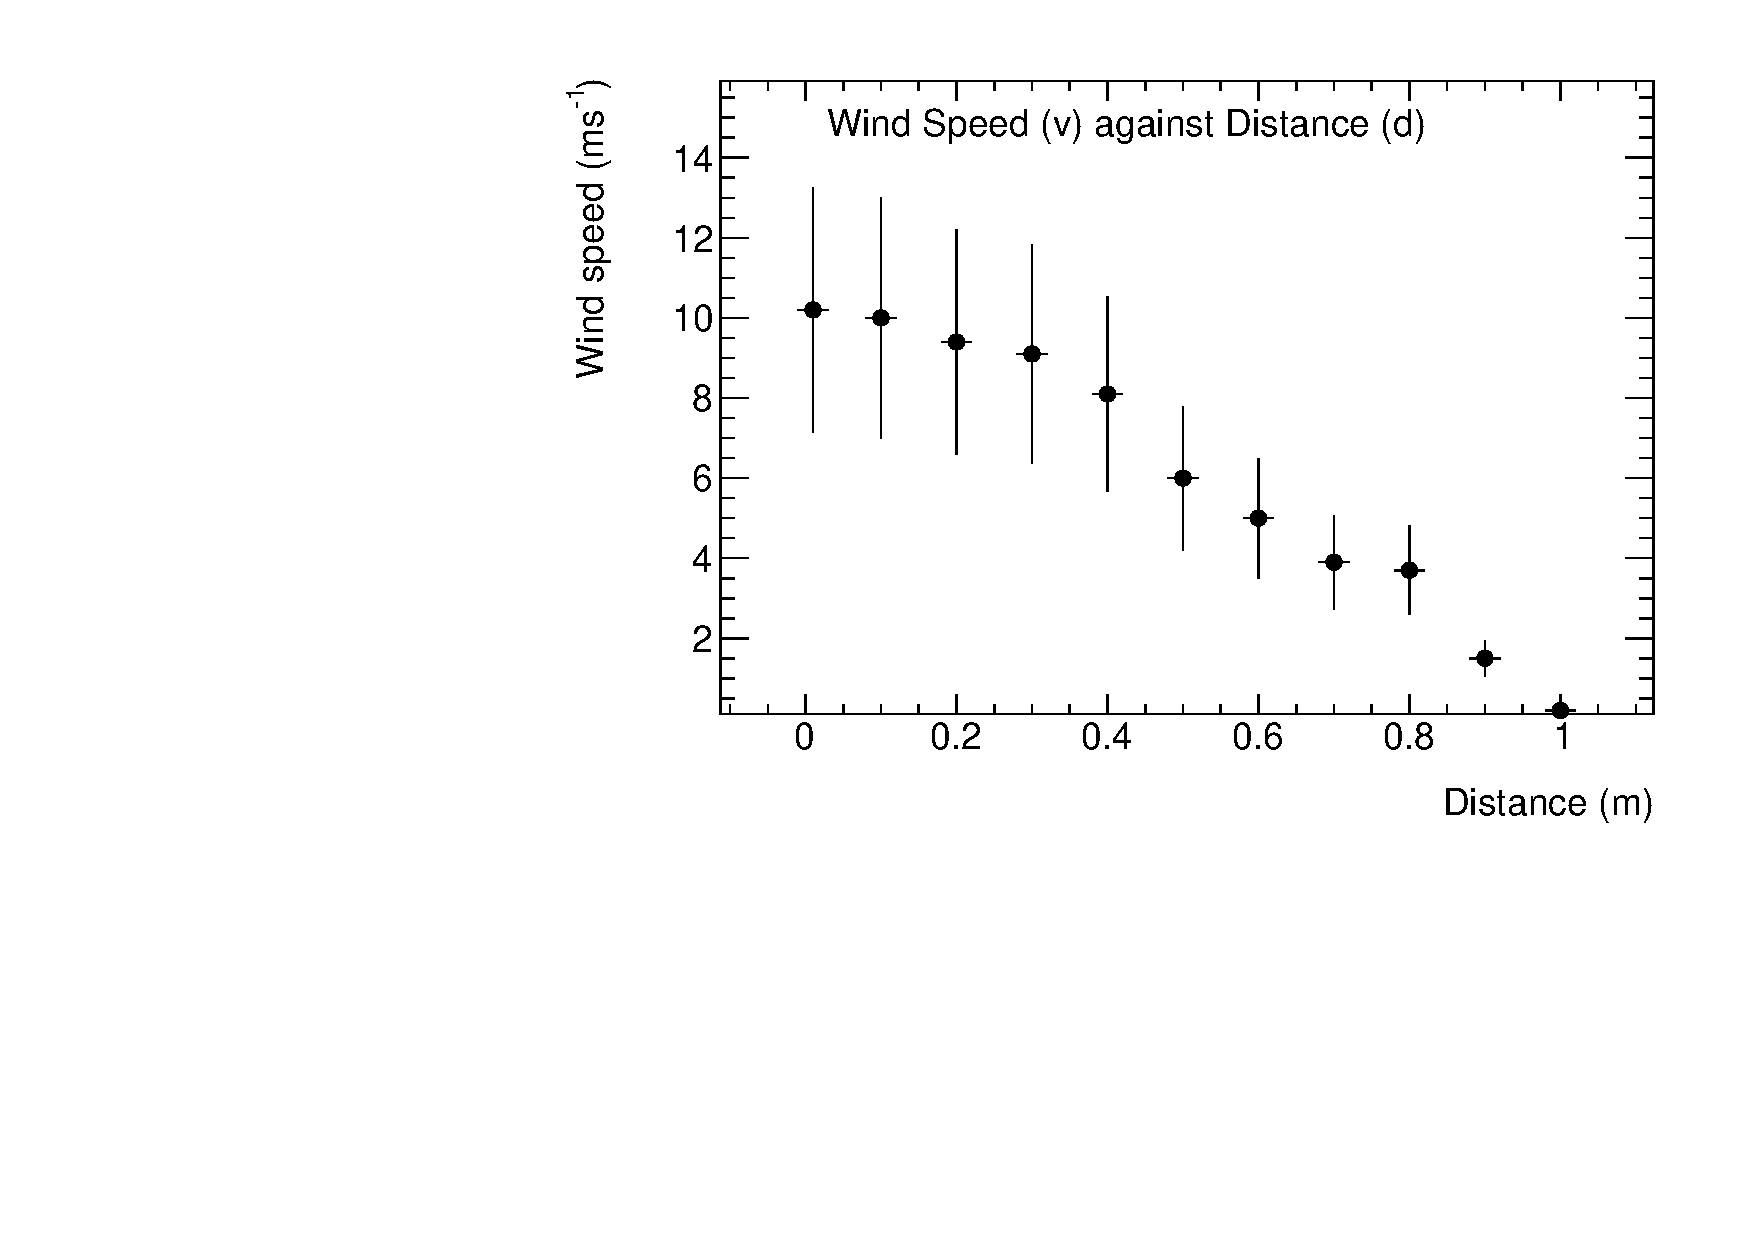
\includegraphics[width=0.5\textwidth]{img/WindSpeedVsDistance.pdf}
\caption{Graph of distance and wind speed}
\label{figure:DistanceVsWindSpeed}
\end{figure}

The fans did not have buttons for regulating the speed, therefore distance was used to control wind speed, and due to air resistance the speed of the air would decrease the longer it has to travel, because it does not have a constant force like an actual wind.
On the graph it can be seen that the larger the distance between the fan and the turbine, the lower the wind speed.

For every \SI{10}{\centi\metre} up to \SI{80}{\centi\metre} I moved the fan and did 20 trials for each distance.
For a trial I pressed `hold' on the voltmeter and the ammeter at the same time every 10 seconds and jotted down the values for each.
Both $V$ and $I$ were measured in \si{\milli\volt} and \si{\milli\ampere}.

For this experiment there was a high risk of having a very large resistance somewhere within the circuit, also in the generator.
However to prove Ohm's law that the resistance is constant if V and I increases proportionally, and to test if the resistance in my circuit was constant, I plotted a graph of current against voltage:

\begin{figure}[h]
\centering
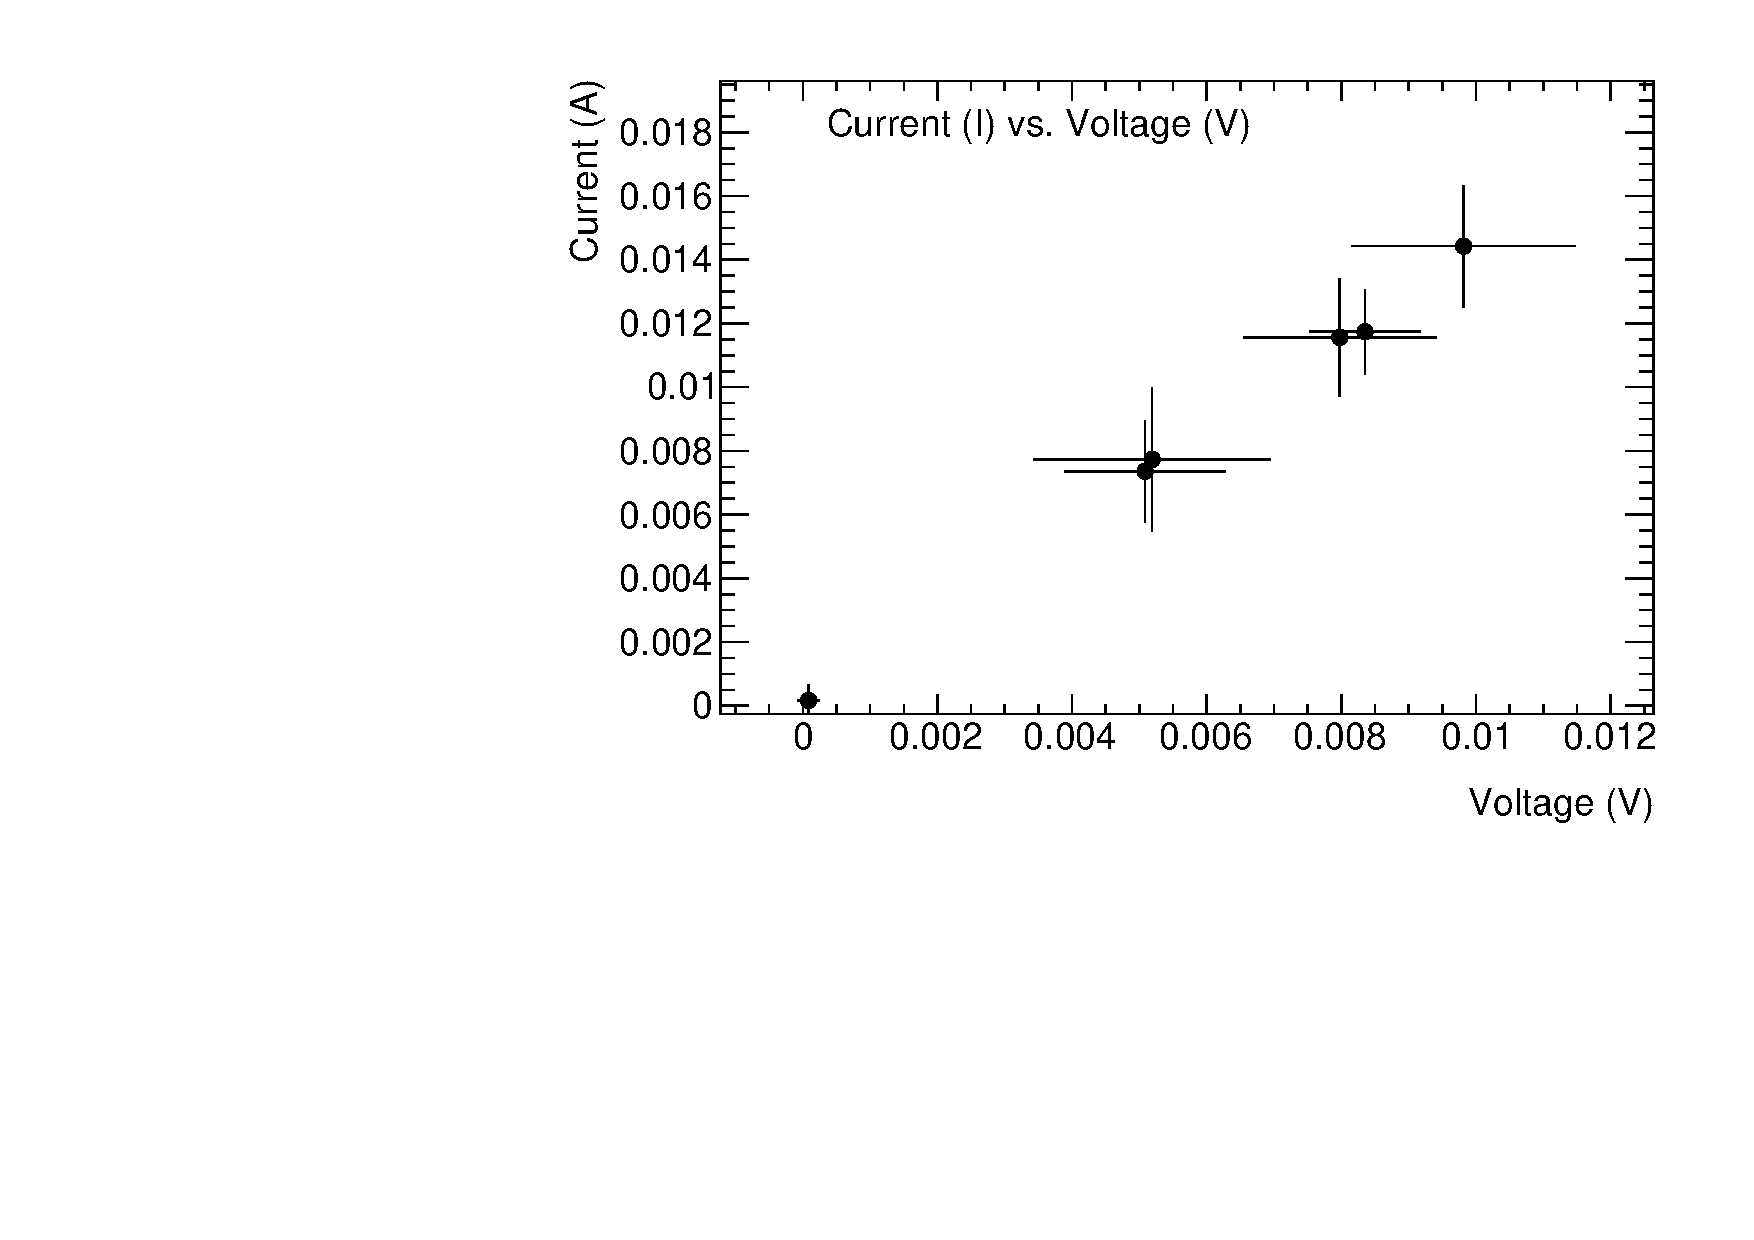
\includegraphics[width=0.5\textwidth]{img/OhmsLaw.pdf}
\caption{Voltage vs current showing a straight line}
\label{figure:OhmsLaw}
\end{figure}

This graph overall represents a straight line with an origin intersecting close to the y-axis at 0.
This graph shows that my data obeys Ohm's law with $I$ and $V$ rising proportionally.
The graph is a check to be sure that the resistance remains the same throughout the experiment and to ensure that the circuit is connected correctly.

For the input power into the turbine, Equation \ref{equation:Windpower} is used.
The radius of the paper blade was measured to \SI{22,5}{\centi\metre}, which gave me the area of the turbine's rotation: $\pi \times 22,5^2 \approx \SI{0,16}{\metre\squared}$.

Then the temperature was measured to $24^o$C and put into a program\cite{AirDensityCalculator}, which calculated the air density; \SI{1,1889}{\kilo\gram\per\metre\cubed}.
With all the variables, I calculated the input power for every different wind speed:

\begin{table}[h]
  \centering
  \begin{tabular}{@{}cc@{}} \toprule
    Average wind speed (\si{\metre\per\second}) & Input power (\si{\watt}) \\ \midrule
    10.2 & 100.3270279 \\
    10.0 & 94.54039917 \\
    9.4 & 78.52374291 \\
    9.1 & 71.24290314 \\
    8.1 & 50.24264428 \\
    6.0 & 20.42072622 \\
    5.0 & 11.8175499 \\
    3.9 & 5.608041938 \\
    3.7 & 0 \\ \bottomrule
\end{tabular}
\caption{A table of the average wind speeds and the calculated input power.}
\label{table:WindSpeedVsPower}
\end{table}

The data is presented on the graph below:

\begin{figure}[h]
  \centering
  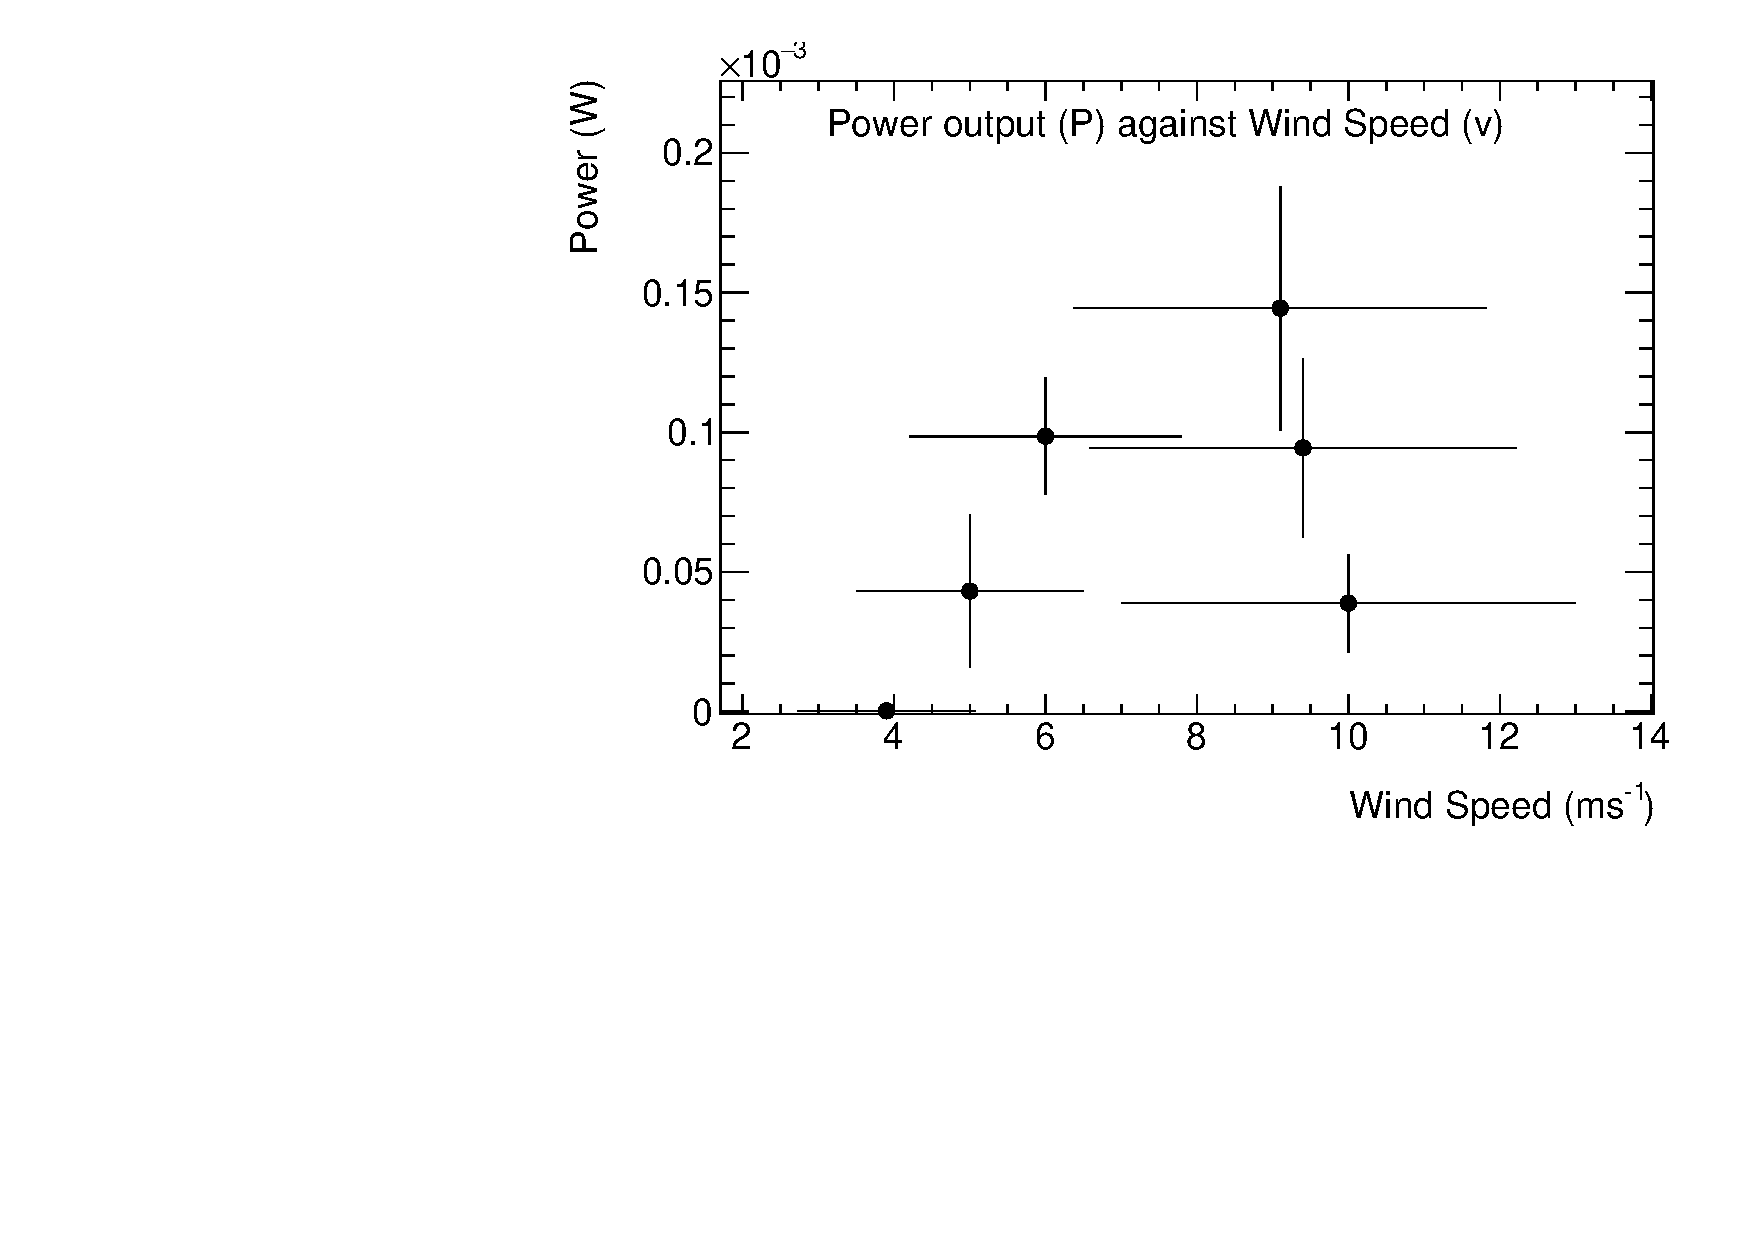
\includegraphics[width=0.5\textwidth]{img/PowerVsWind.pdf}
  \caption{Wind speed vs the output power.}
  \label{figure:final}
\end{figure}

What can be derived from this graph, my turbine starts to produce more power when the wind speed is more than 4 m/s.
However the power outcome also decreases as soon as the wind speed reaches 9m/s and then drops until it reaches 0 W at 10,2 m/s.
When comparing this graph to the wind turbine power graph, mentioned in the section of background theory, it is quite similar in shape to the blue line, since the power outcome increases at a certain speed and decreases at a higher certain speed.
When comparing to that graph, it is important to realise that it is the blue line, since that one represents the effect of stall-regulated wings, and since my turbine cannot pitch its wings and adjust the angle of the blade to the wind, mine would be considered to be stalling throughout the whole experiment.
However, there is a large assumption, which is that along with the highest wind speed is also the shortest distance, which is 0-1 cm and might have been too close for the wind from the fans to move and turn the blades, which might result the 0W for the highest speed.
The fans were placed slightly at an angle to the turbine, since that's how most wind went to the turbine, however that would mean that as the wind turbine is 1-10cm from the fans, the wind did not reach it being out of the area where the air that was almost perpendicular was directed; the stream of air due to the angle did not reach the turbine, meaning that the maximum wind speed had no effect on the turbine and therefore it was 0W.


However, even though this is how much power that comes to the turbine, only a small percentage of this is used and converted in the turbine.
In the background theory it was stated that due to this turbine not being particularly modern nor high tech, a rather low percentage would sound reasonable.

A table was made for every distance measured and voltage and current was noted and power was calculated, which is the output power of the turbine.
Before calculating the mV and mA has to be converted into V and A.

Then I had both input and output in order to calculate the efficiency for each wind speed as shown in Equation \ref{equation:efficiency} using the wind speed 10 m/s:

\begin{equation}
  \epsilon = \frac{\text{input power}}{\text{output power}}
  \label{equation:efficiency}
\end{equation}

%
Rounded off to 3sf the efficiency of the wind speed at 10 m/s is \SI{0,0000253}{\percent}
The rest of the efficiency data is presented in the table below:

\begin{table}[h]
\centering
\begin{tabular}{@{}cc@{}} \toprule
Wind Speed (\si{\metre\per\second}) & Percentage Efficiency ($\times 10^{-5}$) \\ \midrule
10.2 & 0.00 \\ 
10.0 & 1.60 \\ 
9.4  & 3.78 \\ 
9.1  & 5.68 \\ 
6.0  & 8.79 \\ 
5.0  & 21.6 \\ 
3.9  & 0.831 \\ \bottomrule
\end{tabular}
\end{table}

From this table it can be seen that my experiment did not produce any power when the wind speed was at the maximum.
One reason can be that as my turbine was stalling throughout the experiment, as seen on the power curve graph in the background theory, the turbine does not use the extra energy it is provided, but actually decreases it's efficiency.
However the main reason I believe is that as the wind speed was the highest, the distance was as close to 0-1cm from the turbine to the fan, which might have caused the problem that the blades could not catch the wind and therefore the efficiency was 0W, since they did not produce any power and nothing was showing on the volt and ammeter.
It could also be due to the direction of the wind coming from the fans as mentioned earlier.
The reason why the efficiency was \SI{0}{\percent} on wind speeds below 3,7m/s seems reasonable, since the wind speed is rather weak and therefore not strong enough to push the paper blades to make it spin and produce power.


What can be derived from the efficiency data is that the efficiency of my turbine is very low, in fact not even a whole number as a percentage.
It could be expected, since the turbine only produced mV and mA, which are quite small measurements.
Yet, what seemed to be the bigger problem is resistance in the circuit.
In my circuit there was no resistor, since theoretically a resistor would reduce the current and thereby the turbine would produce less power.
What was done here is that the voltmeter was connected across nothing and not a resistor, which might have resulted in the low output.



\section{Uncertainties and Errors}
Since there was collected a lot of data, averages have been used to present the data more simply, which might not have given the most accurate numbers, also counting the data, which is less accurate.
The app measuring wind speed has a conservative uncertainty of 30% based on app calibration.
The voltmeter and ammeter also had uncertainties with .
The temperature has an uncertainty of .
The ruler measuring distance has an uncertainty of , since the construction of the turbine was not straight so the feet on the left side were closer to the fan.
For the area of the blades calculated, the ruler has an uncertainty of  and  
For the input power
\begin{equation}
	\frac{\Delta P}{\Delta P} = \frac{\Delta A}{A} + \frac{\Delta \rho}{\rho} + 3 \frac{\Delta v}{v}
	\label{equation:PowerError}
\end{equation}
I would argue that an error is that the turbine did not function, when the wind speed was the greatest, due to the blade being made of paper not being able to catch the wind.

\section{Conclusion and Evaluation}
My findings of the efficiency of the wind turbine did not seem to fit with the generalised standards of a normal turbine, where a modern high tech turbine can have up to \SI{45}{\percent} efficiency.
This was definitely not the case for my experiment, however the purpose was more to show the way of calculating the efficiency of a turbine.
There is no doubt that my experiment would have a smaller efficiency than actual turbines; my turbine was made at home with a small DC motor designed for a physics investigation and not a supplier for thousands of houses' electricity.

In fact, I was quite impressed that it was able to turn the blades and produce power, even though it was small.
It demonstrates that our unlimited and cost-free air can supply us with energy, and it is therefore a good alternative to fossil fuels.
It was a very interesting field to research and experiment, since it includes so many different aspects of physics such as aerodynamics, mechanics, magnetism, thermal physics, and electricity, which gave me an overview of these aspects and revealed how all these units work together in order to produce the world we have today.


There are many things that can be improved for another investigation.
A more accurate wind speed measuring device can be used.
What can be improved are the thick paper blades of the turbine most particularly; if able to shape the blades with the right angle to the wind instead of just bending them like I did, it would most likely improve the rotation.
Also paper is quite weak, but another material would need to be very light to be able to still rotate.
The fans could also be just one stronger fan instead, limiting the risk of the air velocities to cancel out each other, or being in the wrong direction, which might have been the case for my experiment.
Also the fans had a plastic circle in front and were also protected all around with tiny bars, since it is a fan for a classroom, and shouldn't be blowing super strong air around the room.
If that had not stopped a lot of air from reaching the turbine it might have been a different result.
Also the air might have collided with the bars at an angle and went in another direction cancelling the other fan or complete opposite direction.
An interesting idea is to place a tunnel shaped item from the fans to the turbine, directing the air in the right direction.
Stronger DC motor and better conducting wires could be replaced as well.
What could have been done is to connect a resistor in the circuit and connect the voltmeter across it, which might change the results.
Obviously, more trials for the experiment usually makes the data more accurate even though I did 20 trials for each distance more can be made.



%AGNES: DONT WRITE ANYTHING BELOW HERE

\nocite{*}
\bibliography{references}
\bibliographystyle{unsrt}

%AGNES: PLEASE CHECK THIS STUFF OUT AT THE BOTTOM FOR AN EXPLANATION

%Anything that appears after a '%' is called a 'comment', that means that it will not appear in the PDF version of the document
%Below I have some code that you can copy and paste into your report when you need to:

%EQUATIONS
%This equation has all of the symbols you are likely to use in it, if you need a symbol that isn't written here, ask me or draw it in http://detexify.kirelabs.org/classify.html
%\begin{equation}
%1 + 2 \times 3 \div 4 = \frac{5}{2} = 2.5^{1} 
%\label{WRITE A UNIQUE NAME HERE}
%\end{equation}

%FIGURES
%This will put a figure in the text, the figure doesn't necessarily appear exactly where you will expect it to, but don't worry about that for now.
%Replace the Graph.pdf with your own figure name. Ideally the figures should all be PDF files, but some other image formats also work.
%The figures also have to be in the same folder as the .tex file.
%You can make the picture bigger or smaller by changing the number 0.7 - The maximum size this should be is 1, the smallest size is 0
%\begin{figure}[h]
%  \centering
%  \includegraphics[width=0.7\textwidth]{img/Graph.pdf}
%  \caption{WRITE YOUR CAPTION FOR THE FIGURE HERE}
%  \label{WRITE A UNIQUE NAME HERE}
%\end{figure}

%REFERENCING EQUATIONS AND FIGURES
%If you want to refer to a particular equation or figure in the text, you should write:
%See Figure \ref{UNIQUE NAME HERE THAT CORRESPONDS TO THE NAME IN THE \label{...} OF THE EQUATION OR FIGURE}

%BIBLIOGRAPHY
%If you want to put a reference to the bibliography, you should write:
%...as explained by Albert Einstein \cite{UNIQUE NAME OF REFERENCE}.

%ADDING TO THE BIBLIOGRAPHY LIST
%This is done in the file references.bib, where a full example is given

\end{document}
